\documentclass[border=10pt]{standalone}
% Shared style for the EMONI diagrams. Build: tectonic <file>.tex, then pdftocairo -svg.
\usepackage{fontspec}
\setmainfont{FiraSans}[Extension=.otf,UprightFont=*-Regular,BoldFont=*-SemiBold,ItalicFont=*-Italic,BoldItalicFont=*-SemiBoldItalic]
\setmonofont{FiraMono}[Extension=.otf,UprightFont=*-Regular,BoldFont=*-Medium,Scale=0.9]
\usepackage{tikz}
\usetikzlibrary{arrows.meta,positioning,shapes.geometric,shapes.misc,calc,fit,backgrounds}
\definecolor{eg}{HTML}{11903B}   % EMONI green
\definecolor{egl}{HTML}{E8F7EE}
\definecolor{eb}{HTML}{2A78D6}   % blue
\definecolor{ebl}{HTML}{EAF2FC}
\definecolor{eo}{HTML}{D9631E}   % orange
\definecolor{eol}{HTML}{FDF0E7}
\definecolor{ep}{HTML}{7C4DCC}   % purple
\definecolor{epl}{HTML}{F2ECFB}
\definecolor{er}{HTML}{C5221F}   % red
\definecolor{erl}{HTML}{FCEAEA}
\definecolor{ink}{HTML}{1F2328}
\definecolor{mute}{HTML}{59636E}
\definecolor{line}{HTML}{D0D7DE}
\tikzset{
  every node/.style={text=ink,font=\small},
  >={Stealth[length=2.4mm]},
  % sequence diagrams
  life/.style={draw=line,dashed,thick},
  head/.style={draw=#1,fill=#1!8,rounded corners=3pt,minimum width=27mm,minimum height=11mm,align=center,font=\small\bfseries,thick},
  act/.style={draw=#1,fill=#1!18,minimum width=2.2mm},
  msg/.style={->,thick,draw=ink},
  ret/.style={->,dashed,draw=mute},
  mlabel/.style={font=\footnotesize,fill=white,inner sep=1.5pt,align=center},
  note/.style={draw=#1,fill=#1!8,rounded corners=2pt,font=\footnotesize,align=left,inner sep=4pt},
  frag/.style={draw=mute,rounded corners=2pt},
  fraglabel/.style={draw=mute,fill=white,font=\footnotesize\bfseries,inner sep=2.5pt,anchor=north west},
  % activity diagrams
  start/.style={circle,fill=ink,minimum size=4mm,inner sep=0},
  stop/.style={circle,draw=ink,thick,minimum size=5mm,inner sep=0,path picture={\fill[ink] (path picture bounding box.center) circle (1.4mm);}},
  step/.style={draw=#1,fill=#1!8,rounded corners=5pt,thick,minimum height=9mm,minimum width=40mm,align=center,font=\small},
  step/.default=eg,
  dec/.style={diamond,aspect=2.2,draw=ink,fill=white,thick,inner sep=1.5pt,align=center,font=\footnotesize},
  flow/.style={->,thick,draw=ink},
  guard/.style={font=\footnotesize\itshape,text=mute,fill=white,inner sep=1.5pt},
  lane/.style={draw=line,fill=#1,rounded corners=4pt},
  lanetitle/.style={font=\small\bfseries,text=mute},
}

% Component view of the whole system: devices, networks, the platform, the bench and the clients.
\begin{document}
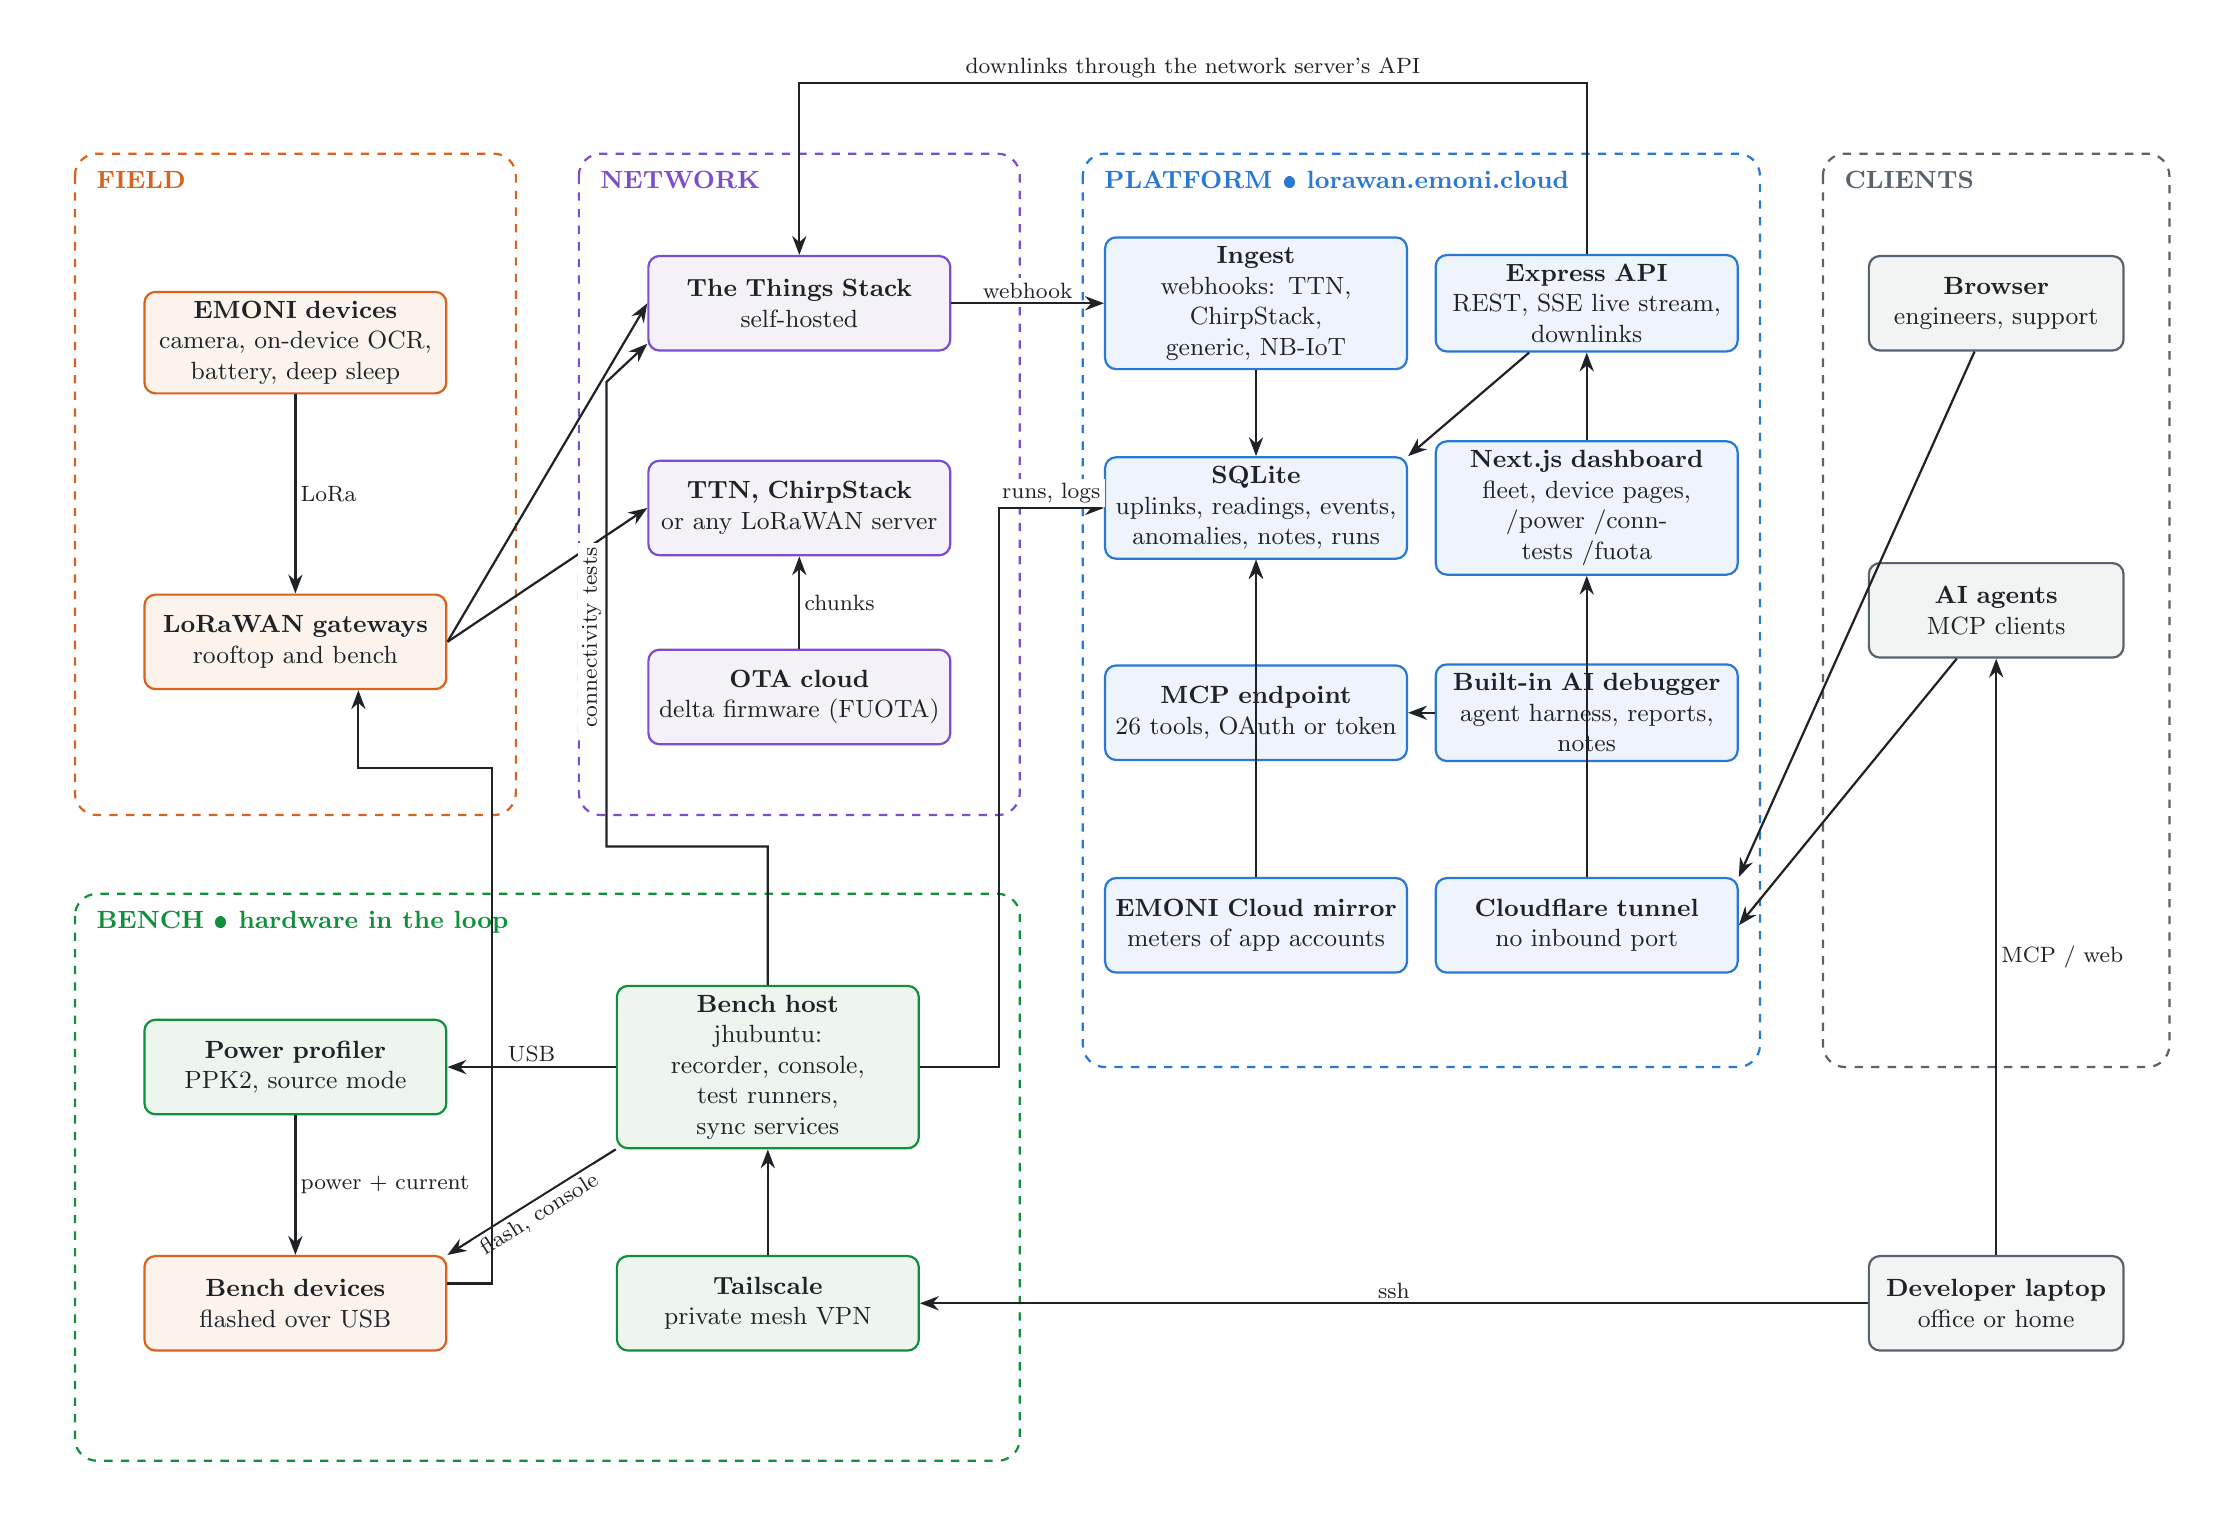
\begin{tikzpicture}[x=1cm,y=1cm]
\tikzset{comp/.style={draw=#1,fill=#1!8,rounded corners=4pt,thick,align=center,minimum height=12mm,text width=36mm,font=\small},
         grp/.style={draw=#1,rounded corners=8pt,dashed,thick},
         gl/.style={font=\small\bfseries,text=#1,anchor=north west},
         lnk/.style={->,thick,draw=ink},
         ll/.style={font=\footnotesize,fill=white,inner sep=1.5pt,align=center}}
\fill[white] (-0.6,1.6) rectangle (27.0,-17.2);
% field
\draw[grp=eo] (0,0) rectangle (5.6,-8.4); \node[gl=eo] at (0.15,-0.1) {FIELD};
\node[comp=eo] (dev) at (2.8,-2.4) {\textbf{EMONI devices}\\camera, on-device OCR,\\battery, deep sleep};
\node[comp=eo] (gw) at (2.8,-6.2) {\textbf{LoRaWAN gateways}\\rooftop and bench};
% network
\draw[grp=ep] (6.4,0) rectangle (12.0,-8.4); \node[gl=ep] at (6.55,-0.1) {NETWORK};
\node[comp=ep] (tts) at (9.2,-1.9) {\textbf{The Things Stack}\\self-hosted};
\node[comp=ep] (other) at (9.2,-4.5) {\textbf{TTN, ChirpStack}\\or any LoRaWAN server};
\node[comp=ep] (ota) at (9.2,-6.9) {\textbf{OTA cloud}\\delta firmware (FUOTA)};
% platform
\draw[grp=eb] (12.8,0) rectangle (21.4,-11.6); \node[gl=eb] at (12.95,-0.1) {PLATFORM \textbullet{} lorawan.emoni.cloud};
\node[comp=eb] (hook) at (15.0,-1.9) {\textbf{Ingest}\\webhooks: TTN, ChirpStack,\\generic, NB-IoT};
\node[comp=eb] (api) at (19.2,-1.9) {\textbf{Express API}\\REST, SSE live stream,\\downlinks};
\node[comp=eb] (db) at (15.0,-4.5) {\textbf{SQLite}\\uplinks, readings, events,\\anomalies, notes, runs};
\node[comp=eb] (ui) at (19.2,-4.5) {\textbf{Next.js dashboard}\\fleet, device pages,\\/power /conn-tests /fuota};
\node[comp=eb] (mcp) at (15.0,-7.1) {\textbf{MCP endpoint}\\26 tools, OAuth or token};
\node[comp=eb] (agent) at (19.2,-7.1) {\textbf{Built-in AI debugger}\\agent harness, reports,\\notes};
\node[comp=eb] (cloud) at (15.0,-9.8) {\textbf{EMONI Cloud mirror}\\meters of app accounts};
\node[comp=eb] (tun) at (19.2,-9.8) {\textbf{Cloudflare tunnel}\\no inbound port};
% bench
\draw[grp=eg] (0,-9.4) rectangle (12.0,-16.6); \node[gl=eg] at (0.15,-9.5) {BENCH \textbullet{} hardware in the loop};
\node[comp=eg] (hil) at (8.8,-11.6) {\textbf{Bench host}\\jhubuntu: recorder, console,\\test runners, sync services};
\node[comp=eg] (ppk) at (2.8,-11.6) {\textbf{Power profiler}\\PPK2, source mode};
\node[comp=eo] (bdev) at (2.8,-14.6) {\textbf{Bench devices}\\flashed over USB};
\node[comp=eg] (ts) at (8.8,-14.6) {\textbf{Tailscale}\\private mesh VPN};
% clients
\draw[grp=mute] (22.2,0) rectangle (26.6,-11.6); \node[gl=mute] at (22.35,-0.1) {CLIENTS};
\node[comp=mute,text width=30mm] (br) at (24.4,-1.9) {\textbf{Browser}\\engineers, support};
\node[comp=mute,text width=30mm] (ai) at (24.4,-5.8) {\textbf{AI agents}\\MCP clients};
\node[comp=mute,text width=30mm] (lap) at (24.4,-14.6) {\textbf{Developer laptop}\\office or home};
% links
\draw[lnk] (dev) -- node[ll,right]{LoRa} (gw);
\draw[lnk] (gw.east) -- (tts.west);
\draw[lnk] (gw.east) -- (other.west);

\draw[lnk] (tts.east) -- node[ll,above]{webhook} (hook.west);

\draw[lnk] (api.north) -- (19.2,0.9) -- node[ll,above]{downlinks through the network server's API} (9.2,0.9) -- (tts.north);
\draw[lnk] (ota) -- node[ll,right]{chunks} (other);
\draw[lnk] (hook) -- (db); \draw[lnk] (api) -- (db.north east);
\draw[lnk] (ui) -- (api); \draw[lnk] (mcp) -- (db); \draw[lnk] (agent) -- (mcp); \draw[lnk] (cloud) -- (db);
\draw[lnk] (br) -- (tun.north east);
\draw[lnk] (ai) -- (tun.east);
\draw[lnk] (tun) -- (ui);
\draw[lnk] (hil) -- node[ll,above]{USB} (ppk);
\draw[lnk] (ppk) -- node[ll,right]{power + current} (bdev);
\draw[lnk] (hil.south west) -- node[ll,sloped,below]{flash, console} (bdev.north east);
\draw[lnk] ($(bdev.east)+(0,0.25)$) -- (5.3,-14.35) -- (5.3,-7.8) -| ($(gw.south)+(0.8,0)$);
\draw[lnk] (hil.east) -- ++(1.0,0) |- node[ll,pos=0.75,above]{runs, logs} (db.west);
\draw[lnk] (hil.north) -- (8.8,-8.8) -- (6.75,-8.8) -- node[ll,sloped,above,pos=0.45]{connectivity tests} (6.75,-2.9) -- ($(tts.south west)+(0,0.1)$);
\draw[lnk] (lap.west) -- node[ll,above]{ssh} (ts.east);
\draw[lnk] (ts) -- (hil);
\draw[lnk] (lap.north) -- node[ll,right]{MCP / web} (ai.south);
\end{tikzpicture}
\end{document}
